\subsection{COMPLEX CIRCULAR FUNCTIONS; HYPERBOLIC FUNCTIONS}

Euler's formulae (25) (III, p.~99) and the definition of \(e^z\) for every complex \(z\) allow us to extend to \(\mathbf{C}\) the functions \(\cos x\) and \(\sin x\) defined on \(\mathbf{R}\) , by putting, for all \(z \in \mathbf{C}\)

\[
\cos z = \frac {1}{2} \left(e ^ {i z} + e ^ {- i z}\right), \quad \sin z = \frac {1}{2 i} \left(e ^ {i z} - e ^ {- i z}\right)\tag{32}
\]

(cf.~III, p.~119, exerc. 19).

These functions are periodic with principal period \(2\pi\) ; that is, one has \(\cos(z + \pi/2) = -\sin z\) , \(\sin(z + \pi/2) = \cos z\) ; one may also verify the identities

\[
\begin{array}{c} \cos^ {2} z + \sin^ {2} z = 1 \\ \cos (z + z ^ {\prime}) = \cos z \cos z ^ {\prime} - \sin z \sin z ^ {\prime} \\ \sin (z + z ^ {\prime}) = \sin z \cos z ^ {\prime} + \cos z \sin z ^ {\prime}. \end{array}
\]

More generally, every algebraic identity between circular functions for real variables remains true when one gives these variables arbitrary complex values (III, p.~119, exerc. 18).

One puts \(\tan z = \sin z/\cos z\) if \(z \neq (2k + 1)\pi/2\) and \(\cot z = \cos z/\sin z\) if \(z \neq k\pi\) ; these are periodic functions with principal period \(\pi\) .

Formula (27) (III, p.~99) shows that \(\cos z\) and \(\sin z\) are differentiable on \(\mathbf{C}\) , and that

\[
\mathrm{D} (\cos z) = - \sin z, \quad \mathrm{D} (\sin z) = \cos z.
\]

For \(z = ix\) (x real), the formulae (32) give

\[
\cos i x = \frac {1}{2} \left(e ^ {x} + e ^ {- x}\right), \quad \sin i x = \frac {i}{2} \left(e ^ {x} - e ^ {- x}\right).
\]

It is convenient to have a specific notation for the real functions thus introduced; we put

\[
\left\{ \begin{array}{l l} \cosh x = \frac {1}{2} \left(e ^ {x} + e ^ {- x}\right) & \text {(hyperbolic cosine of x)} \\ \sinh x = \frac {i}{2} \left(e ^ {x} - e ^ {- x}\right) & \text {(hyperbolic sine of x)} \\ \tanh x = \frac {\sinh x}{\cosh x} = \frac {e ^ {x} - e ^ {- x}}{e ^ {x} + e ^ {- x}} & \text {(hyperbolic tangent of x)} \end{array} \right.\tag{33}
\]

One thus has, for every real \(x\)

\[
\cos i x = \cosh x, \quad \sin i x = i \sinh x.\tag{34}
\]

From every identity between circular functions in a certain number of complex numbers \(z_{k}\) ( \(1 \leqslant k \leqslant n\) ) one can deduce an identity for the hyperbolic functions, by replacing \(z_{k}\) by \(ix_{k}\) ( \(x_{k}\) real, \(1 \leqslant k \leqslant n\) ) and using the formulae (34); for instance one has

\[
\begin{array}{c} \cosh^ {2} x - \sinh^ {2} x = 1 \\ \cosh (x + x ^ {\prime}) = \cosh x \cosh x ^ {\prime} + \sinh x \sinh x ^ {\prime} \\ \sinh (x + x ^ {\prime}) = \sinh x \cosh x ^ {\prime} - \cosh x \sinh x ^ {\prime}. \end{array}
\]

The hyperbolic functions allow us to express the real and imaginary parts of \(\cos z\) and \(\sin z\) for \(z = x + iy\) , since

\[
\begin{array}{l} \cos (x + i y) = \cos x \cos i y - \sin x \sin i y = \cos x \cosh y - i \sin x \sinh y \\ \sin (x + i y) = \sin x \cos i y + \cos x \sin i y = \sin x \cosh y + i \cos x \sinh y. \end{array}
\]

Finally, one has

\[
\mathrm{D} (\cosh x) = \sinh x, \mathrm{D} (\sinh x) = \cosh x, \mathrm{D} (\tanh x) = 1 - \tanh ^ {2} x = \frac {1}{\cosh^ {2} x}.
\]

Since \(\cosh x > 0\) for all x one deduces that \(\sinh x\) is strictly increasing on R; since \(\sinh 0 = 0\) , it follows that \(\sinh x\) has the same sign as x. In consequence \(\cosh x\) is strictly decreasing for \(x \leqslant 0\) , strictly increasing for \(x \geqslant 0\) ; finally, \(\tanh x\) is strictly increasing on R. Moreover

\[
\begin{array}{l} \lim _ {x \to - \infty} \sinh x = - \infty , \quad \lim _ {x \to + \infty} \sinh x = + \infty \\ \lim _ {x \to - \infty} \cosh x = \lim _ {x \to + \infty} \cosh x = + \infty \\ \lim _ {x \to - \infty} \tanh x = - 1, \quad \lim _ {x \to + \infty} \tanh x = + 1 \quad (\text {   fig.   8   and   9   }). \end{array}
\]

Sometimes we write \(\operatorname{Arg}\sinh x\) for the inverse function of \(\sinh x\) , which is a strictly increasing map from \(\mathbf{R}\) onto \(\mathbf{R}\) ; this function can also be expressed in terms of the logarithm, since from the relation \(x = \sinh y = \frac{1}{2}(e^y - e^{-y})\) we deduce that \(e^{2y} - 2xe^y - 1 = 0\) , and since \(e^y > 0\) , we have \(e^y = x + \sqrt{x^2 + 1}\) , that is to say

\[
\operatorname{Arg} \sinh x = \log (x + \sqrt {x ^ {2} + 1}).
\]

Similarly, we denote by \(\operatorname{Arg}\cosh x\) the inverse of the restriction of \(\cosh x\) to \([0, +\infty[\) ; this map is strictly increasing from \([1, +\infty[\) onto \([0, +\infty[\) ; one shows as above that

\[
\operatorname{Arg} \cosh x = \log (x + \sqrt {x ^ {2} - 1}).
\]

\pandocbounded{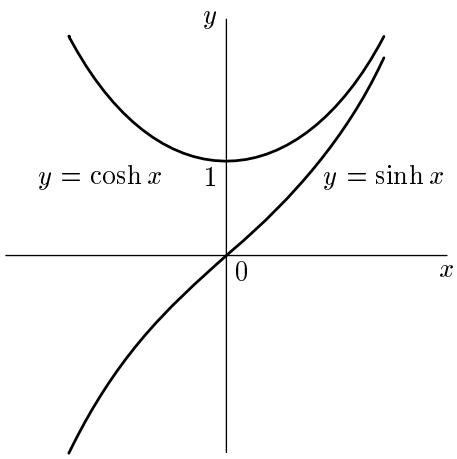
\includegraphics[keepaspectratio]{images/part001_d9e35212.jpg}}\\
Fig. 8

\pandocbounded{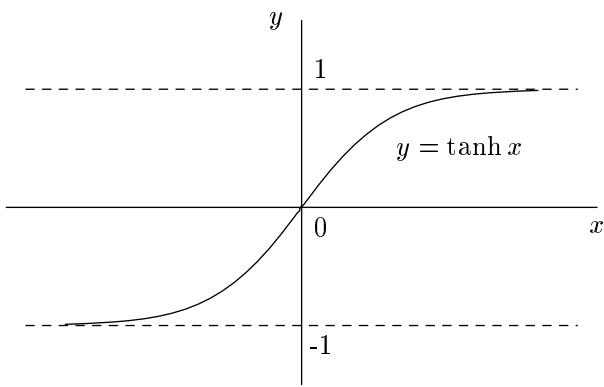
\includegraphics[keepaspectratio]{images/part001_f5896466.jpg}}\\
Fig. 9

Finally, we denote by \(\operatorname{Arg}\tanh x\) the inverse function of \(\tanh x\) , which is a strictly increasing map from \(] - 1, +1[\) onto \(\mathbf{R}\) ; one has, moreover,

\[
\operatorname{Arg} \tanh x = \frac {1}{2} \log \frac {1 + x}{1 - x}.
\]

Remark. For complex \(z\) one sometimes writes

\[
\begin{array}{l} \cosh z = \frac {1}{2} (e ^ {z} + e ^ {- z}) = \cos i z \\ \sinh z = \frac {1}{2} (e ^ {z} - e ^ {- z}) = - i \sin i z. \end{array}
\]

These functions thus extend to C the hyperbolic functions defined on R.

